\phantomsection
\addcontentsline{toc}{chapter}{Appendices}

% The \appendix command resets the chapter counter, and changes the chapter numbering scheme to capital letters.
%\chapter{Appendices}
\appendix

\chapter{pyKrack}
\label{appendix:pykrack}

CAHpter on pykrack as a package. Concept of hierachy in a graph. Krackhadt heirahrcy. 

Implementaiotn in Python

Compare against already existing R implemtnation.
using nbdev for coding, vignettes, documentation, packaging and plublishing (to pypi).

Some kind of figure here

\section{Introduction}

Biological signaling can be modeled as a directed network, where nodes represent genes/proteins and edges represent signaling interactions.

The hierarchy of such a network can be quantified using various metrics, including the Krackhardt hierarchy score. This score measures the degree to which the network exhibits a perfect hierarchy, with higher scores indicating greater hierarchy.

In R the sna package presents methods to compute graph hierarchy including Krackhardt’s score (defined as
where is the number of unordered pairs of points in Dr that are asymmetrically linked), and there are other hierarchy scores implemented in Python such as Flow Hierarchy Score Luo and Magee 2011. However, despite its utility, there is currently no native implementation of the Krackhardt hierarchy score in Python.

\subsection{Krackhardt hierarchy score}

As defined in Krackhardt, David. (1994). Graph Theoretical Dimensions of Informal Organization. Computational Organization Theory. 89.

The graph hierarchy condition states that in a digraph D, for each pair of points where one (Pi) can reach another (Pj), the second (Pj) can't reach the first (Pi). 
For example, in a formal organization chart a high lvl employee can reach through the chain of command her subordinate's subordinate. If the formal organization is working "properly", this lower lvl employee can't simultaneously reach the high lvl employee.
To measure the degree of hierarchy of digraph D, a new digraph Dr must be created. Dr is defined as the reachability digraph of D. Each point in D exists in Dr; moreover, the line (Pi,Pj) exists in Dr if and only if Pi can reach Pj in D. If D is graph hierarchic, then Dr will have no symmetric lines in it (i.e. if the line (Pi,Pj) exists in Dr then the line (Pj,Pi) does not).

The degree of hierarchy then is defined as:

Where is the number of unordered pairs of points in Dr that are symmetrically linked , and the number of unordered pairs of points in Dr where Pi is linked to Pj or viceversa.

%%%%%%%%

The Krackhardt hierarchy score is given by the following equation:

\begin{equation}
H_i = \frac{\sum_{j \in P_i} w_{ij} H_j}{k_i}
\end{equation}

where $H_i$ is the hierarchy score for node $i$, $P_i$ is the set of direct reports of node $i$, $w_{ij}$ is the weight of the edge between nodes $i$ and $j$, and $k_i$ is the number of direct reports of node $i$.

This equation calculates the hierarchy score for each node in a network based on the hierarchy scores of its direct reports and the weights of the edges between them. The hierarchy score represents the level of influence or power that a node has in the network, with higher scores indicating greater influence.


\section{Implementation}

\subsection{compute hierarchy function}

\subsection{nbdev paltform}




\chapter{Supplementary Figures}
\label{appendix:SupFig}

\section{Figures related to Chapter \ref{04seq}}

\begin{figure}[h!]
    \centering
    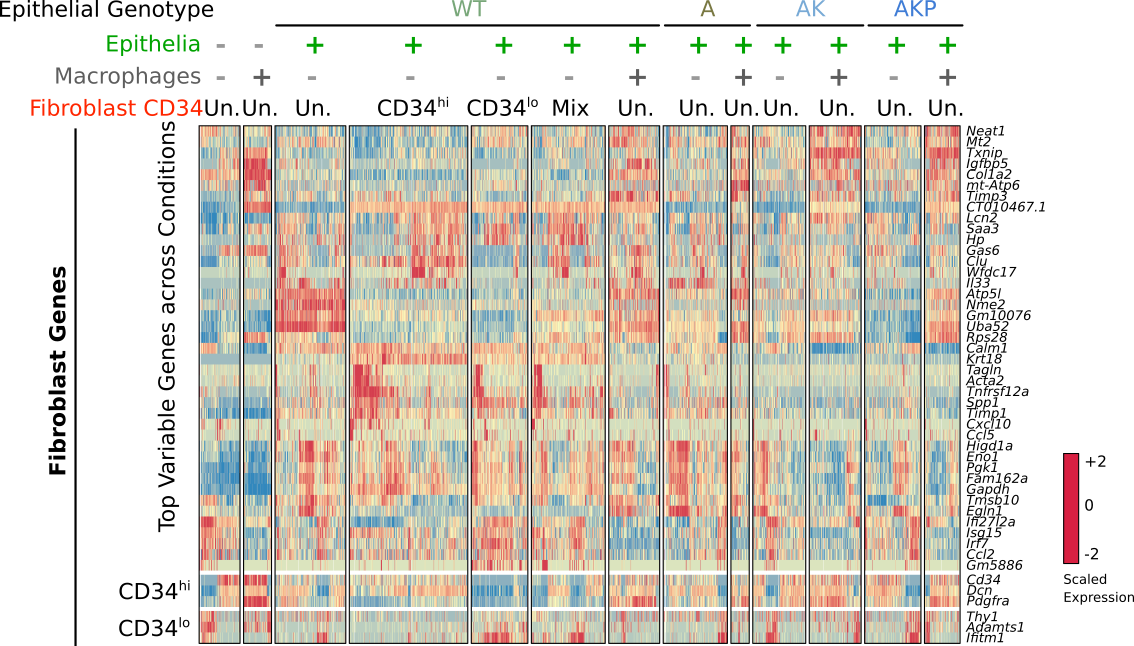
\includegraphics{0Xappendices/0XSup_DEfib.png}
    \caption{}
    \label{sfig:defib}
\end{figure}

\begin{figure}[h!]
    \centering
    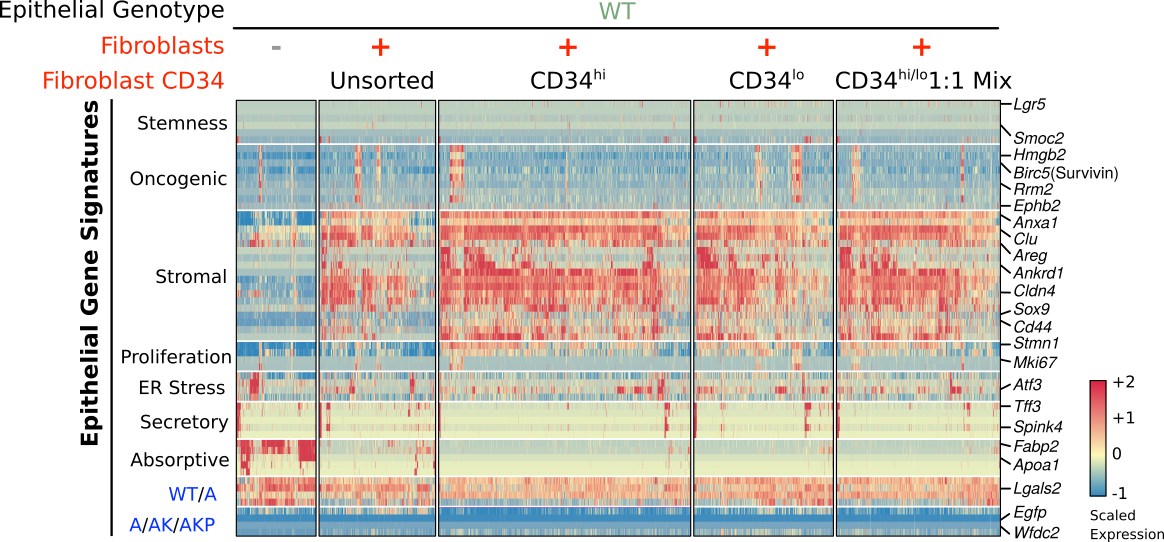
\includegraphics{0Xappendices/0XSup_DEepibyfib.png}
    \caption{}
    \label{sfig:deepibyfib}
\end{figure}

\begin{figure}[h!]
    \centering
    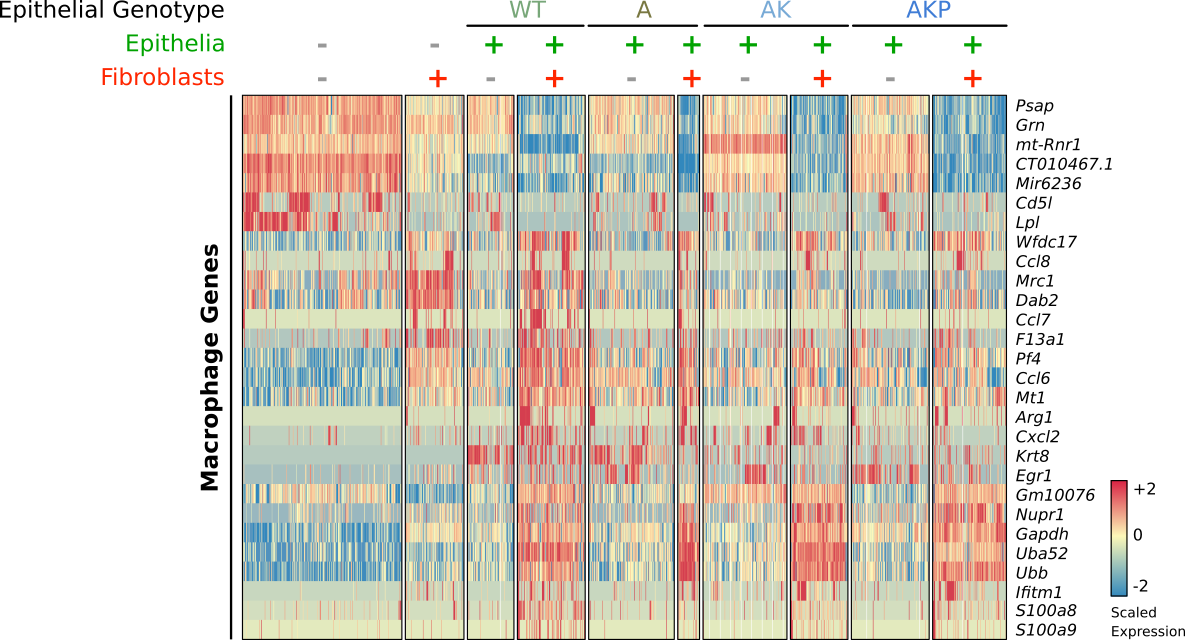
\includegraphics{0Xappendices/0XSup_DEmac.png}
    \caption{}
    \label{sfig:demac}
\end{figure}

\chapter{Supplementary Tables}
\label{appendix:SupTab}

\section{Gene Data}

\newpage
\begin{table}[H]
  \centering
  \caption{\textbf{Colonic epithelia gene markers (1/2)}. MArkers of epithelia populatin and orgnaoid genotypes. Derived from literature and DE analysis of our data.}
  \label{tab:epimarkers}
  \csvreader[
    tabular=|c|c|,
    head=true,
    table head=\hline \textbf{Gene} & \textbf{Annotation}\\ \hline,
    late after line=\\ \hline,
    filter={\value{csvinputline}<30},
    separator=comma,
    respect all
  ]{0Xappendices/CuratedEpithelia_geneSet.csv}{}
  {\csvcoli & \csvcolii}
\end{table}
\newpage
\begin{table}[H]
  \centering
  \caption{\textbf{Colonic epithelia gene markers (2/2)}.}
  \csvreader[
    tabular=|c|c|,
    head=true,
    table head=\hline \textbf{Gene} & \textbf{Annotation}\\ \hline,
    late after line=\\ \hline,
    filter={\value{csvinputline}>29},
    separator=comma,
    respect all
  ]{0Xappendices/CuratedEpithelia_geneSet.csv}{}
  {\csvcoli & \csvcolii}
\end{table}

\newpage
\begin{table}[H]
  \centering
  \caption{\textbf{Cell-cycle gene lists (1/6)}. Table of cell-cycle genes adapted from Tirosh et al. 2016 \cite{tirosh_dissecting_2016} and Macosko et al. 2015 \cite{macosko_highly_2015}, the former using a human melanoma cell line and the later both human and mouse models to link gene expression with cell cycle phases. The original tables provided in the publication were pooled together, duplicated genes were dropped, and human symbols were translated to mouse using BioMart. Finally, genes whose expression could not be detected in any of the mouse organoid experiments were dropped from the list. The resulting table contains 98 genes associated with S-phase, 248 with both G2 and M-phase, and 202 with G1.}
  \csvreader[
    tabular=|c|c|c|,
    table head=\hline \textbf{S-phase} & \textbf{G2 \& M-phase} & \textbf{G1} \\ \hline,
    late after line=\\ \hline,
    filter={\value{csvinputline}<39},
    separator=tab
  ]{0Xappendices/CellCycle_geneSet.txt}{}%
  {\csvcoli & \csvcolii & \csvcoliii}
  % \caption{Your table caption}
  \label{tab:cycle}
\end{table}
\newpage
\begin{table}[H]
  \centering
  \caption{\textbf{Cell-cycle gene lists (2/6)}.}
  \csvreader[
    tabular=|c|c|c|,
    table head=\hline \textbf{S-phase} & \textbf{G2 \& M-phase} & \textbf{G1} \\ \hline,
    late after line=\\ \hline,
    filter expr={
      test{\ifnumgreater{\thecsvinputline}{38}}
  and test{\ifnumless{\thecsvinputline}{82}}},
    separator=tab
  ]{0Xappendices/CellCycle_geneSet.txt}{}%
  {\csvcoli & \csvcolii & \csvcoliii}
\end{table}
\newpage
\begin{table}[H]
  \centering
  \caption{\textbf{Cell-cycle gene lists (3/6)}.}
  \csvreader[
    tabular=|c|c|c|,
    table head=\hline \textbf{S-phase} & \textbf{G2 \& M-phase} & \textbf{G1} \\ \hline,
    late after line=\\ \hline,
    filter expr={
      test{\ifnumgreater{\thecsvinputline}{81}}
  and test{\ifnumless{\thecsvinputline}{125}}},
    separator=tab
  ]{0Xappendices/CellCycle_geneSet.txt}{}%
  {\csvcoli & \csvcolii & \csvcoliii}
\end{table}
\newpage
\begin{table}[H]
  \centering
  \caption{\textbf{Cell-cycle gene lists (4/6)}.}
  \csvreader[
    tabular=|c|c|c|,
    table head=\hline \textbf{S-phase} & \textbf{G2 \& M-phase} & \textbf{G1} \\ \hline,
    late after line=\\ \hline,
    filter expr={
      test{\ifnumgreater{\thecsvinputline}{124}}
  and test{\ifnumless{\thecsvinputline}{168}}},
    separator=tab
  ]{0Xappendices/CellCycle_geneSet.txt}{}%
  {\csvcoli & \csvcolii & \csvcoliii}
\end{table}
\newpage
\begin{table}[H]
  \centering
  \caption{\textbf{Cell-cycle gene lists (5/6)}.}
  \csvreader[
    tabular=|c|c|c|,
    table head=\hline \textbf{S-phase} & \textbf{G2 \& M-phase} & \textbf{G1} \\ \hline,
    late after line=\\ \hline,
    filter expr={
      test{\ifnumgreater{\thecsvinputline}{167}}
  and test{\ifnumless{\thecsvinputline}{211}}},
    separator=tab
  ]{0Xappendices/CellCycle_geneSet.txt}{}%
  {\csvcoli & \csvcolii & \csvcoliii}
\end{table}
\newpage
\begin{table}[H]
  \centering
  \caption{\textbf{Cell-cycle gene lists (6/6)}.}
  \csvreader[
    tabular=|c|c|c|,
    table head=\hline \textbf{S-phase} & \textbf{G2 \& M-phase} & \textbf{G1} \\ \hline,
    late after line=\\ \hline,
    filter expr={
      test{\ifnumgreater{\thecsvinputline}{210}}},
    separator=tab
  ]{0Xappendices/CellCycle_geneSet.txt}{}%
  {\csvcoli & \csvcolii & \csvcoliii}
  % \caption{Your table caption}
\end{table}

\newpage
\begin{table}[H]
  \centering
  \caption{\textbf{Literature gene signatures (1/2)}. In the context of Stem states of the intestinal and colon epithelia.}
  \label{tab:SignMD}
  \csvreader[
    tabular=|c|c|c|c|c|,
    head=true,
    table head=\hline \textbf{Name} & \textbf{Genes} & \textbf{Context} & \textbf{Species} & \textbf{Reference} \\ \hline,
    late after line=\\ \hline,
    filter={\value{csvinputline}<37},
    separator=comma,
    respect all
  ]{0Xappendices/SignMD.csv}{}
  {\csvcoli & \csvcolii & \csvcoliii & \csvcoliv & \csvcolv}
\end{table}
\newpage
\begin{table}[H]
  \centering
  \caption{\textbf{Literature gene signature (2/2)}.}
  \csvreader[
    tabular=|c|c|c|c|c|,
    head=true,
    table head=\hline \textbf{Name} & \textbf{Genes} & \textbf{Context} & \textbf{Species} & \textbf{Reference} \\ \hline,
    late after line=\\ \hline,
    filter={\value{csvinputline}>36},
    separator=comma,
    respect all
  ]{0Xappendices/SignMD.csv}{}
  {\csvcoli & \csvcolii & \csvcoliii & \csvcoliv & \csvcolv}
\end{table}

\newpage
\newpage
\newpage
\section{Knowledge Graph Data}

\label{tab:wavpy}
\lstinputlisting[language=Python, caption=\textbf{Wavelet module}. Script kindly provided by Aarthi Venkat from Prof. Smita Krishnaswamy's lab at Yale University., firstline=35, lastline=65]{0Xappendices/localization.py}

\begin{sidewaystable}
    \centering
    \caption{GEx dist}
    \label{tab:kgdistge}
    \begin{tabular}{lrrrrrrrrrr}
        {} & {ER Stress} & {E. Entero.} & {L. Entero.} & {Secret.} & {proCSC} & {CSC} & {TA2} & {revCSC} & {TA1} & {Fibroblast} \\
        ER Stress & {\cellcolor[HTML]{000004}} \color[HTML]{F1F1F1} 0.000000 & {\cellcolor[HTML]{240C4F}} \color[HTML]{F1F1F1} 0.134136 & {\cellcolor[HTML]{120A32}} \color[HTML]{F1F1F1} 0.087232 & {\cellcolor[HTML]{280B53}} \color[HTML]{F1F1F1} 0.144213 & {\cellcolor[HTML]{310A5C}} \color[HTML]{F1F1F1} 0.161209 & {\cellcolor[HTML]{2D0B59}} \color[HTML]{F1F1F1} 0.154001 & {\cellcolor[HTML]{CE4347}} \color[HTML]{F1F1F1} 0.553933 & {\cellcolor[HTML]{230C4C}} \color[HTML]{F1F1F1} 0.129671 & {\cellcolor[HTML]{3D0965}} \color[HTML]{F1F1F1} 0.187844 & {\cellcolor[HTML]{FA9207}} \color[HTML]{000000} 0.759904 \\
        E. Entero. & {\cellcolor[HTML]{240C4F}} \color[HTML]{F1F1F1} 0.134136 & {\cellcolor[HTML]{000004}} \color[HTML]{F1F1F1} 0.000000 & {\cellcolor[HTML]{1B0C41}} \color[HTML]{F1F1F1} 0.110047 & {\cellcolor[HTML]{320A5E}} \color[HTML]{F1F1F1} 0.166665 & {\cellcolor[HTML]{3B0964}} \color[HTML]{F1F1F1} 0.185258 & {\cellcolor[HTML]{380962}} \color[HTML]{F1F1F1} 0.177877 & {\cellcolor[HTML]{D74B3F}} \color[HTML]{F1F1F1} 0.580909 & {\cellcolor[HTML]{2D0B59}} \color[HTML]{F1F1F1} 0.153192 & {\cellcolor[HTML]{470B6A}} \color[HTML]{F1F1F1} 0.211384 & {\cellcolor[HTML]{FCA50A}} \color[HTML]{000000} 0.797288 \\
        L. Entero. & {\cellcolor[HTML]{120A32}} \color[HTML]{F1F1F1} 0.087232 & {\cellcolor[HTML]{1B0C41}} \color[HTML]{F1F1F1} 0.110047 & {\cellcolor[HTML]{000004}} \color[HTML]{F1F1F1} 0.000000 & {\cellcolor[HTML]{1C0C43}} \color[HTML]{F1F1F1} 0.116684 & {\cellcolor[HTML]{260C51}} \color[HTML]{F1F1F1} 0.139993 & {\cellcolor[HTML]{230C4C}} \color[HTML]{F1F1F1} 0.132073 & {\cellcolor[HTML]{CB4149}} \color[HTML]{F1F1F1} 0.543032 & {\cellcolor[HTML]{190C3E}} \color[HTML]{F1F1F1} 0.106004 & {\cellcolor[HTML]{320A5E}} \color[HTML]{F1F1F1} 0.164687 & {\cellcolor[HTML]{FCA108}} \color[HTML]{000000} 0.790359 \\
        Secret. & {\cellcolor[HTML]{280B53}} \color[HTML]{F1F1F1} 0.144213 & {\cellcolor[HTML]{320A5E}} \color[HTML]{F1F1F1} 0.166665 & {\cellcolor[HTML]{1C0C43}} \color[HTML]{F1F1F1} 0.116684 & {\cellcolor[HTML]{000004}} \color[HTML]{F1F1F1} 0.000000 & {\cellcolor[HTML]{400A67}} \color[HTML]{F1F1F1} 0.197554 & {\cellcolor[HTML]{3D0965}} \color[HTML]{F1F1F1} 0.189356 & {\cellcolor[HTML]{DE5238}} \color[HTML]{F1F1F1} 0.604088 & {\cellcolor[HTML]{310A5C}} \color[HTML]{F1F1F1} 0.162743 & {\cellcolor[HTML]{4A0C6B}} \color[HTML]{F1F1F1} 0.221462 & {\cellcolor[HTML]{FAC62D}} \color[HTML]{000000} 0.864652 \\
        proCSC & {\cellcolor[HTML]{310A5C}} \color[HTML]{F1F1F1} 0.161209 & {\cellcolor[HTML]{3B0964}} \color[HTML]{F1F1F1} 0.185258 & {\cellcolor[HTML]{260C51}} \color[HTML]{F1F1F1} 0.139993 & {\cellcolor[HTML]{400A67}} \color[HTML]{F1F1F1} 0.197554 & {\cellcolor[HTML]{000004}} \color[HTML]{F1F1F1} 0.000000 & {\cellcolor[HTML]{440A68}} \color[HTML]{F1F1F1} 0.203334 & {\cellcolor[HTML]{DB503B}} \color[HTML]{F1F1F1} 0.596904 & {\cellcolor[HTML]{390963}} \color[HTML]{F1F1F1} 0.180319 & {\cellcolor[HTML]{510E6C}} \color[HTML]{F1F1F1} 0.237957 & {\cellcolor[HTML]{FB9906}} \color[HTML]{000000} 0.776085 \\
        CSC & {\cellcolor[HTML]{2D0B59}} \color[HTML]{F1F1F1} 0.154001 & {\cellcolor[HTML]{380962}} \color[HTML]{F1F1F1} 0.177877 & {\cellcolor[HTML]{230C4C}} \color[HTML]{F1F1F1} 0.132073 & {\cellcolor[HTML]{3D0965}} \color[HTML]{F1F1F1} 0.189356 & {\cellcolor[HTML]{440A68}} \color[HTML]{F1F1F1} 0.203334 & {\cellcolor[HTML]{000004}} \color[HTML]{F1F1F1} 0.000000 & {\cellcolor[HTML]{DA4E3C}} \color[HTML]{F1F1F1} 0.592524 & {\cellcolor[HTML]{360961}} \color[HTML]{F1F1F1} 0.173165 & {\cellcolor[HTML]{4F0D6C}} \color[HTML]{F1F1F1} 0.230962 & {\cellcolor[HTML]{FB9B06}} \color[HTML]{000000} 0.781164 \\
        TA2 & {\cellcolor[HTML]{CE4347}} \color[HTML]{F1F1F1} 0.553933 & {\cellcolor[HTML]{D74B3F}} \color[HTML]{F1F1F1} 0.580909 & {\cellcolor[HTML]{CB4149}} \color[HTML]{F1F1F1} 0.543032 & {\cellcolor[HTML]{DE5238}} \color[HTML]{F1F1F1} 0.604088 & {\cellcolor[HTML]{DB503B}} \color[HTML]{F1F1F1} 0.596904 & {\cellcolor[HTML]{DA4E3C}} \color[HTML]{F1F1F1} 0.592524 & {\cellcolor[HTML]{000004}} \color[HTML]{F1F1F1} 0.000000 & {\cellcolor[HTML]{D44842}} \color[HTML]{F1F1F1} 0.573983 & {\cellcolor[HTML]{E55C30}} \color[HTML]{F1F1F1} 0.630285 & {\cellcolor[HTML]{FCFFA4}} \color[HTML]{000000} 1.000000 \\
        revCSC & {\cellcolor[HTML]{230C4C}} \color[HTML]{F1F1F1} 0.129671 & {\cellcolor[HTML]{2D0B59}} \color[HTML]{F1F1F1} 0.153192 & {\cellcolor[HTML]{190C3E}} \color[HTML]{F1F1F1} 0.106004 & {\cellcolor[HTML]{310A5C}} \color[HTML]{F1F1F1} 0.162743 & {\cellcolor[HTML]{390963}} \color[HTML]{F1F1F1} 0.180319 & {\cellcolor[HTML]{360961}} \color[HTML]{F1F1F1} 0.173165 & {\cellcolor[HTML]{D44842}} \color[HTML]{F1F1F1} 0.573983 & {\cellcolor[HTML]{000004}} \color[HTML]{F1F1F1} 0.000000 & {\cellcolor[HTML]{440A68}} \color[HTML]{F1F1F1} 0.206725 & {\cellcolor[HTML]{FC9F07}} \color[HTML]{000000} 0.787210 \\
        TA1 & {\cellcolor[HTML]{3D0965}} \color[HTML]{F1F1F1} 0.187844 & {\cellcolor[HTML]{470B6A}} \color[HTML]{F1F1F1} 0.211384 & {\cellcolor[HTML]{320A5E}} \color[HTML]{F1F1F1} 0.164687 & {\cellcolor[HTML]{4A0C6B}} \color[HTML]{F1F1F1} 0.221462 & {\cellcolor[HTML]{510E6C}} \color[HTML]{F1F1F1} 0.237957 & {\cellcolor[HTML]{4F0D6C}} \color[HTML]{F1F1F1} 0.230962 & {\cellcolor[HTML]{E55C30}} \color[HTML]{F1F1F1} 0.630285 & {\cellcolor[HTML]{440A68}} \color[HTML]{F1F1F1} 0.206725 & {\cellcolor[HTML]{000004}} \color[HTML]{F1F1F1} 0.000000 & {\cellcolor[HTML]{FBB61A}} \color[HTML]{000000} 0.835137 \\
        Fibroblast & {\cellcolor[HTML]{FA9207}} \color[HTML]{000000} 0.759904 & {\cellcolor[HTML]{FCA50A}} \color[HTML]{000000} 0.797288 & {\cellcolor[HTML]{FCA108}} \color[HTML]{000000} 0.790359 & {\cellcolor[HTML]{FAC62D}} \color[HTML]{000000} 0.864652 & {\cellcolor[HTML]{FB9906}} \color[HTML]{000000} 0.776085 & {\cellcolor[HTML]{FB9B06}} \color[HTML]{000000} 0.781164 & {\cellcolor[HTML]{FCFFA4}} \color[HTML]{000000} 1.000000 & {\cellcolor[HTML]{FC9F07}} \color[HTML]{000000} 0.787210 & {\cellcolor[HTML]{FBB61A}} \color[HTML]{000000} 0.835137 & {\cellcolor[HTML]{000004}} \color[HTML]{F1F1F1} 0.000000 \\
    \end{tabular}
\end{sidewaystable}

\begin{sidewaystable}
    \centering
    \caption{LRT dist}
    \label{tab:kgdistlrt}
    \begin{tabular}{lrrrrrrrrrr}
        {} & {ER Stress} & {E. Entero.} & {L. Entero.} & {Secret.} & {proCSC} & {CSC} & {TA2} & {revCSC} & {TA1} & {Fibroblast} \\
        ER Stress & {\cellcolor[HTML]{000004}} \color[HTML]{F1F1F1} 0.000000 & {\cellcolor[HTML]{490B6A}} \color[HTML]{F1F1F1} 0.215563 & {\cellcolor[HTML]{290B55}} \color[HTML]{F1F1F1} 0.145190 & {\cellcolor[HTML]{260C51}} \color[HTML]{F1F1F1} 0.139818 & {\cellcolor[HTML]{420A68}} \color[HTML]{F1F1F1} 0.201897 & {\cellcolor[HTML]{490B6A}} \color[HTML]{F1F1F1} 0.218083 & {\cellcolor[HTML]{E55C30}} \color[HTML]{F1F1F1} 0.632105 & {\cellcolor[HTML]{400A67}} \color[HTML]{F1F1F1} 0.198838 & {\cellcolor[HTML]{62146E}} \color[HTML]{F1F1F1} 0.277580 & {\cellcolor[HTML]{FCA60C}} \color[HTML]{000000} 0.803968 \\
        E. Entero. & {\cellcolor[HTML]{490B6A}} \color[HTML]{F1F1F1} 0.215563 & {\cellcolor[HTML]{000004}} \color[HTML]{F1F1F1} 0.000000 & {\cellcolor[HTML]{2D0B59}} \color[HTML]{F1F1F1} 0.153977 & {\cellcolor[HTML]{290B55}} \color[HTML]{F1F1F1} 0.147012 & {\cellcolor[HTML]{470B6A}} \color[HTML]{F1F1F1} 0.211975 & {\cellcolor[HTML]{4D0D6C}} \color[HTML]{F1F1F1} 0.227420 & {\cellcolor[HTML]{E9612B}} \color[HTML]{F1F1F1} 0.647468 & {\cellcolor[HTML]{450A69}} \color[HTML]{F1F1F1} 0.209010 & {\cellcolor[HTML]{65156E}} \color[HTML]{F1F1F1} 0.287032 & {\cellcolor[HTML]{FCB418}} \color[HTML]{000000} 0.828309 \\
        L. Entero. & {\cellcolor[HTML]{290B55}} \color[HTML]{F1F1F1} 0.145190 & {\cellcolor[HTML]{2D0B59}} \color[HTML]{F1F1F1} 0.153977 & {\cellcolor[HTML]{000004}} \color[HTML]{F1F1F1} 0.000000 & {\cellcolor[HTML]{0D0829}} \color[HTML]{F1F1F1} 0.074063 & {\cellcolor[HTML]{280B53}} \color[HTML]{F1F1F1} 0.143724 & {\cellcolor[HTML]{2F0A5B}} \color[HTML]{F1F1F1} 0.159109 & {\cellcolor[HTML]{D94D3D}} \color[HTML]{F1F1F1} 0.587539 & {\cellcolor[HTML]{260C51}} \color[HTML]{F1F1F1} 0.138559 & {\cellcolor[HTML]{490B6A}} \color[HTML]{F1F1F1} 0.217404 & {\cellcolor[HTML]{FCA60C}} \color[HTML]{000000} 0.802999 \\
        Secret. & {\cellcolor[HTML]{260C51}} \color[HTML]{F1F1F1} 0.139818 & {\cellcolor[HTML]{290B55}} \color[HTML]{F1F1F1} 0.147012 & {\cellcolor[HTML]{0D0829}} \color[HTML]{F1F1F1} 0.074063 & {\cellcolor[HTML]{000004}} \color[HTML]{F1F1F1} 0.000000 & {\cellcolor[HTML]{260C51}} \color[HTML]{F1F1F1} 0.138364 & {\cellcolor[HTML]{2D0B59}} \color[HTML]{F1F1F1} 0.153222 & {\cellcolor[HTML]{D84C3E}} \color[HTML]{F1F1F1} 0.583433 & {\cellcolor[HTML]{240C4F}} \color[HTML]{F1F1F1} 0.132827 & {\cellcolor[HTML]{470B6A}} \color[HTML]{F1F1F1} 0.211676 & {\cellcolor[HTML]{FCA60C}} \color[HTML]{000000} 0.803792 \\
        proCSC & {\cellcolor[HTML]{420A68}} \color[HTML]{F1F1F1} 0.201897 & {\cellcolor[HTML]{470B6A}} \color[HTML]{F1F1F1} 0.211975 & {\cellcolor[HTML]{280B53}} \color[HTML]{F1F1F1} 0.143724 & {\cellcolor[HTML]{260C51}} \color[HTML]{F1F1F1} 0.138364 & {\cellcolor[HTML]{000004}} \color[HTML]{F1F1F1} 0.000000 & {\cellcolor[HTML]{450A69}} \color[HTML]{F1F1F1} 0.210823 & {\cellcolor[HTML]{E35933}} \color[HTML]{F1F1F1} 0.621495 & {\cellcolor[HTML]{3E0966}} \color[HTML]{F1F1F1} 0.194830 & {\cellcolor[HTML]{5F136E}} \color[HTML]{F1F1F1} 0.271929 & {\cellcolor[HTML]{FA9207}} \color[HTML]{000000} 0.761176 \\
        CSC & {\cellcolor[HTML]{490B6A}} \color[HTML]{F1F1F1} 0.218083 & {\cellcolor[HTML]{4D0D6C}} \color[HTML]{F1F1F1} 0.227420 & {\cellcolor[HTML]{2F0A5B}} \color[HTML]{F1F1F1} 0.159109 & {\cellcolor[HTML]{2D0B59}} \color[HTML]{F1F1F1} 0.153222 & {\cellcolor[HTML]{450A69}} \color[HTML]{F1F1F1} 0.210823 & {\cellcolor[HTML]{000004}} \color[HTML]{F1F1F1} 0.000000 & {\cellcolor[HTML]{E8602D}} \color[HTML]{F1F1F1} 0.640803 & {\cellcolor[HTML]{470B6A}} \color[HTML]{F1F1F1} 0.211221 & {\cellcolor[HTML]{65156E}} \color[HTML]{F1F1F1} 0.288502 & {\cellcolor[HTML]{FCA108}} \color[HTML]{000000} 0.790591 \\
        TA2 & {\cellcolor[HTML]{E55C30}} \color[HTML]{F1F1F1} 0.632105 & {\cellcolor[HTML]{E9612B}} \color[HTML]{F1F1F1} 0.647468 & {\cellcolor[HTML]{D94D3D}} \color[HTML]{F1F1F1} 0.587539 & {\cellcolor[HTML]{D84C3E}} \color[HTML]{F1F1F1} 0.583433 & {\cellcolor[HTML]{E35933}} \color[HTML]{F1F1F1} 0.621495 & {\cellcolor[HTML]{E8602D}} \color[HTML]{F1F1F1} 0.640803 & {\cellcolor[HTML]{000004}} \color[HTML]{F1F1F1} 0.000000 & {\cellcolor[HTML]{E45A31}} \color[HTML]{F1F1F1} 0.627242 & {\cellcolor[HTML]{F37819}} \color[HTML]{F1F1F1} 0.703030 & {\cellcolor[HTML]{FCFFA4}} \color[HTML]{000000} 1.000000 \\
        revCSC & {\cellcolor[HTML]{400A67}} \color[HTML]{F1F1F1} 0.198838 & {\cellcolor[HTML]{450A69}} \color[HTML]{F1F1F1} 0.209010 & {\cellcolor[HTML]{260C51}} \color[HTML]{F1F1F1} 0.138559 & {\cellcolor[HTML]{240C4F}} \color[HTML]{F1F1F1} 0.132827 & {\cellcolor[HTML]{3E0966}} \color[HTML]{F1F1F1} 0.194830 & {\cellcolor[HTML]{470B6A}} \color[HTML]{F1F1F1} 0.211221 & {\cellcolor[HTML]{E45A31}} \color[HTML]{F1F1F1} 0.627242 & {\cellcolor[HTML]{000004}} \color[HTML]{F1F1F1} 0.000000 & {\cellcolor[HTML]{5F136E}} \color[HTML]{F1F1F1} 0.270369 & {\cellcolor[HTML]{FCA80D}} \color[HTML]{000000} 0.807421 \\
        TA1 & {\cellcolor[HTML]{62146E}} \color[HTML]{F1F1F1} 0.277580 & {\cellcolor[HTML]{65156E}} \color[HTML]{F1F1F1} 0.287032 & {\cellcolor[HTML]{490B6A}} \color[HTML]{F1F1F1} 0.217404 & {\cellcolor[HTML]{470B6A}} \color[HTML]{F1F1F1} 0.211676 & {\cellcolor[HTML]{5F136E}} \color[HTML]{F1F1F1} 0.271929 & {\cellcolor[HTML]{65156E}} \color[HTML]{F1F1F1} 0.288502 & {\cellcolor[HTML]{F37819}} \color[HTML]{F1F1F1} 0.703030 & {\cellcolor[HTML]{5F136E}} \color[HTML]{F1F1F1} 0.270369 & {\cellcolor[HTML]{000004}} \color[HTML]{F1F1F1} 0.000000 & {\cellcolor[HTML]{F9C932}} \color[HTML]{000000} 0.873586 \\
        Fibroblast & {\cellcolor[HTML]{FCA60C}} \color[HTML]{000000} 0.803968 & {\cellcolor[HTML]{FCB418}} \color[HTML]{000000} 0.828309 & {\cellcolor[HTML]{FCA60C}} \color[HTML]{000000} 0.802999 & {\cellcolor[HTML]{FCA60C}} \color[HTML]{000000} 0.803792 & {\cellcolor[HTML]{FA9207}} \color[HTML]{000000} 0.761176 & {\cellcolor[HTML]{FCA108}} \color[HTML]{000000} 0.790591 & {\cellcolor[HTML]{FCFFA4}} \color[HTML]{000000} 1.000000 & {\cellcolor[HTML]{FCA80D}} \color[HTML]{000000} 0.807421 & {\cellcolor[HTML]{F9C932}} \color[HTML]{000000} 0.873586 & {\cellcolor[HTML]{000004}} \color[HTML]{F1F1F1} 0.000000 \\
    \end{tabular}

\end{sidewaystable}

% \chapter{Cell-state Random Forest Classifier}
% \label{appendix:rfclass}

% \section*{Rationale and Aims}

% The maturity of the platform is also reflected on the properties of the markers used in the mass cytometry panels, with the most robust markers achieving highly binary and specific staining. Given the importance of cell state changes to perturbations in the epithelial organoids, either in the form of intrinsic effects such as genotype or extrinsic in the form of the TME or drug treatments, an automated approach of labelling and assigning a cell state to each cell in an experiment would facilitate routine analysis of mass cytometry datasets. 
% I thus hypothesise that we can use a machine learning approach to, using a series of canonical cell state markers, automatically predict and label the hundreds of thousands of cells captured in a mass cytometry experiment. To this end I aim to develop a random-forest classifier. This classifier will be able to ingest mass cytometry datasets and, using manually gated datasets with cell state labels as training data, label each of the cells with one of six possible cell states: Apoptosis, G0, G1, S-phase, G2, and M-phase. 

% \section*{Implementation}
% The cell state classifier built uses the scikit-learn Python package35 to train and run a Random Forest classification algorithm. A Random Forest algorithm (referred to as RF hereafter) is based on a series of decision trees, simple non-parametric models that predict the class of an observation by learning decision rules inferred from the data during training. By using a randomised collection of these trees (i.e., a forest) the RF palliates the tendency of decision trees towards overfitness while at the same time reducing the variance of the results.

% The current implementation in my personal GitHub repository (https://github.com/FerranC96/C\_StateML) consists of two scripts written in Python that are able to 1) train and save RF models from pre-labelled datasets, and generate classification reports and plots, 2) run the saved RF models through new mass cytometry datasets to label and assign a state to each cells. Default parameters are used for the Random Forest (except for an increase in the number of decision trees to 480) and the data is transformed as usual using an arcsinh function with a cofactor of 5. 

% Some of the results presented in this document correspond to an initial implementation of the RF algorithm that used only 5 different cell state markers: pRB [S807/S811], cleaved Caspase 3 [D175], IdU, Cyclin B1, and pHH3 [S28]. This 5-marker implementation was trained using a balanced subset of cells from SI LGR5 time-course experiment in Qin et al. 202011 (downsampled so that all six cell states would have the same number of cells, 5306). The trained model was then tested against datasets from the same publication; a simpler single-timepoint SI LGR5 culture, and a complex coculture of colonic organoids (with varying degrees of CRC mutations and TME complexity).
% In contrast, the latest results use data acquired from Patient Derived Organoids of CRC patients. With an updated panel, the markers used in the latest models are a set of ten antibodies (the five markers from above plus cPARP [D214], pAKT [T308], pP38 [T180/Y182], Geminin, and PLK1) with targets specific to each of the six cell state classes (Apoptosis, G0, G1, S-phase, G2, and M-phase). This 10-marker model was trained on an untreated control condition replicate and testing is performed against a second set of replicates comprising a total of 5 conditions (plus an untreated control) treated with increasing concentration of the chemotherapeutic topoisomerase inhibitor SN-38.
% Details on the markers used in the RF models, and the cell state they are associated with, can be found in Sup. Table 1. To benchmark the model performance, we use F1-scores (calculated as the harmonic mean of the precision and recall for each class).

% \section*{Results}

% Testing the 5-marker RF model on a single time-point SI LGR5 organoid culture11 results in global accuracy for all classes of 0.93. However, looking at the classification report in Figure 3 a) we see how there is a significant drop of f1-scores when classifying the apoptotic class, scores which otherwise remain above 0.92. This fall in f1-scores seems to be driven by a low precision (0.5) when classifying cells as apoptotic.
% Performance of the classifier drops when testing against the CRC TME colonic organoid cultures from Qin et al. 2020. In this case, when we subset just the organoid cells from the organoid cultures (i.e., by extracting all epithelial cells irrespective of the genotype or the other cell types they might have been analysed with), we observe a global accuracy of 0.91. Looking at the classification details (Figure 3 b.) we see a very similar pattern to the SI LGR5 results; with the apoptotic class presenting the lowest f1-scores (0.6) characterised by a low precision (0.43). Furthermore, the remaining f1-scores are also lower overall, with only the S-phase and M-phase classes reaching above the 0.9 mark.
% When instead of subsetting just the organoid cells we test against all cells from the CRC TME dataset (i.e., including also fibroblasts and macrophages) global accuracy drops down to 0.87. The relatively high global accuracy does not reflect the failure of the classifier to, yet again, identify the apoptotic cells (see Figure 3 c.). In Figure 3 d) the classification matrix is used to build a dot plot in which the true labels (“Real state” from gating) are compared against the predicted labels (“Predicted state”), highlighting how a majority of the cells labelled as apoptotic are actually G0 cells, explaining the precision of 0.32 for the former class. There is also some confusion around the G2 cells, as a significant number of these cells are classified as either G0 or G1.
 
% Figure 3: Benchmarking 5-marker RF cell state classifier. Shown in a), b), and c) are the classification reports obtained from running the 5-marker RF classifier against data manually labelled for cell state (representing the “real state” or ground truth). In a) a single timepoint SI LGR5 dataset was used, very similar to the training data for the model. The dataset in both b) and c) is a coculture of CRC organoids and their TME, with the cells in b) being a subset of the whole dataset containing just epithelial cells. Decreasing levels of performance correlate with increasing differences between the train and test datasets, as can be seen by the low f1-scores for the apoptotic class in c). Using the same data as c), the dot plot derived from the classification matrix in d) depicts the number and proportion (as both size and colour of the circles) of mislabelled cells for each cell state, showing that a considerable number of falsely mislabelled apoptotic cells are actually in G0 phase and some cells. RF: Random Forest.
% Preliminary benchmark results from the updated 10-marker implementation using PDO data show improved performance when compared to the 5-marker model. In this case we observe a global accuracy greater than 0.99, with the lowest f1-score being of 0.95 for the cells in M-phase (see Figure 4 a.). In the classification matrix in Figure 4 b) we observe how, given the lower total count of M-phase cells (true label = 5, one order of magnitude smaller than the other classes), small numbers of misclassified cells (mainly as G2 and S-phase predicted labels, represented by the numbers 4 and 3 respectively) drive down the recall for the M-phase class. 
% In contrast with the 5-marker model results, there is an apparent lack of issues when classifying the apoptotic class, with only 0.35% of true apoptotic cells being mislabelled. A bar plot representing the importance of each feature during classification is shown in Sup. Figure 2.
 
% Figure 4: Benchmarking the new 10-marker RF cell state classifier. Building a RF classifier with an increased number of markers using data from PDOs renders better results than the original 5-marker model, as can be seen in a) with the classification report. b) Classification matrix generated automatically during model building, showing extremely low levels of misclassified cells. RF: Random Forest. PDO: Patient-Derived Organoids. Labels: 0=Apoptosis, 1=G0, 2=G1, 3=S-phase, 4=G2, 5=M-phase.


% \section*{Discussion}
% This classifier shows link PTM->cellSTate, later shown in pubs from our lab
% Usefullness in determining antibodies not working properly?


\chapter{CardosoRodriguez \& Qin et al. 2023}
\label{appendix:XXX}

\includepdf[pages=-, scale=1, offset=24mm -28mm]{0Xappendices/preprint.pdf}



\chapter{Colophon}
\label{appendix3label}
\textit{This is a description of the tools you used to make your thesis. It helps people make future documents, reminds you, and looks good.}

Thesis made in latex. Figures assembled in the open source vecotr editing software Inkscape. Resources using for making figures include plots generated from code, de-novo graphics, and graphics altered from the open source Bioicons resource. 

This Thesis is currently hosted in GitHub as a private repository, but as soon as the sections of work currently under revision at Cell are part of the public domain I will make the repository public. Code availability covers all Chapters and is distributed along multiple GitHub repositories.

\textit{(example)} This document was set in the Times Roman typeface using \LaTeX\ and Bib\TeX , composed with a text editor. 
 % description of document, e.g. type faces, TeX used, TeXmaker, packages and things used for figures. Like a computational details section.
% e.g. http://tex.stackexchange.com/questions/63468/what-is-best-way-to-mention-that-a-document-has-been-typeset-with-tex#63503

% Side note:
%http://tex.stackexchange.com/questions/1319/showcase-of-beautiful-typography-done-in-tex-friends
